\chapter{Graficzny interfejs aplikacji}
\label{chapter:chapter_gui}

\section{Strona główna}

Strona główna aplikacji Ebook-Wizard (patrz: Rysunek \ref{fig:page_main}) jest dostępna pod adresem \href{https://ebookwizard.danielrogowski.net/}{https://ebookwizard.danielrogowski.net/}. Jest to w założeniu pierwsza strona, którą odwiedzi nowy użytkownik aplikacji. Na stronie głównej zaprezentowane są podstawowe informacje na temat aplikacji - lista najważniejszych funkcji, wykaz wspieranych rozszerzeń plików i zachęta do założenia konta w serwisie.

Jeśli użytkownik nie jest jeszcze zalogowany, na stronie głównej wyświetlają się przyciski nawigujące do formularzy logowania i rejestracji. Jeśli użytkownik jest już uwierzytelniony, zamiast tego na stronie głównej wyświetla się przycisk "Otwórz mój dysk".


\begin{figure}[h]
    \centering
    \setlength{\fboxsep}{0pt}
    \setlength{\fboxrule}{0.4pt}
    \fbox{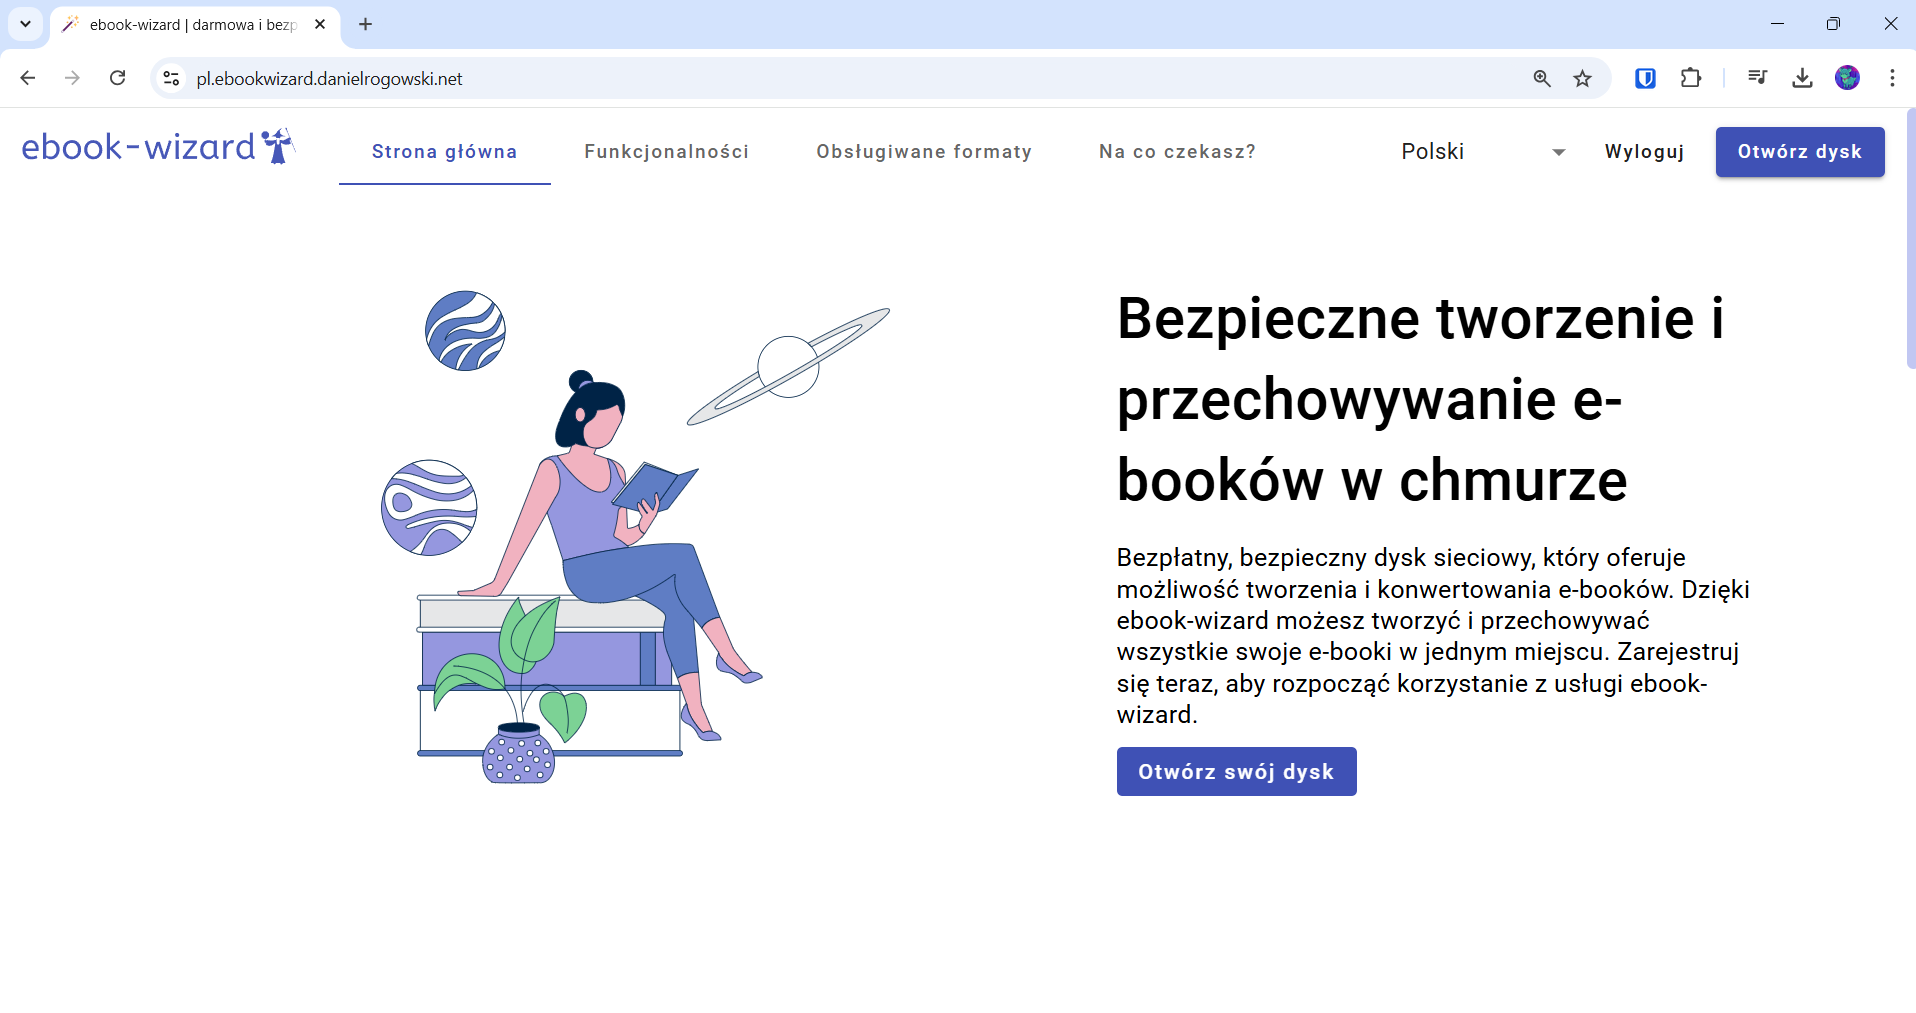
\includegraphics[width=0.9\textwidth]{chap4/page_home.png}}
    \caption{Strona główna aplikacji Ebook-Wizard}
    \label{fig:page_main}
\end{figure}

W przypadku, gdy użytkownik odwiedzi stronę z urządzenia o małym ekranie (na przykład smartfonu), strona główna dostosowuje swoją zawartość, co zaprezentowano na Rysunku \ref{fig:page_main_mobile}. Ozdobne ilustracje zostają usunięte, aby zrobić miejsce dla tekstu i przycisków nawigujących. Ponadto, poziome menu na samej górze strony zostaje zwinięte do postaci menu bocznego, wysuwanego po wciśnięciu przycisku.

\begin{figure}[h]
    \centering
    \setlength{\fboxsep}{0pt}
    \setlength{\fboxrule}{0.4pt}
    \fbox{
\includegraphics[width=0.3\textwidth]{chap4/page_home_andrut.jpg}}
    \caption{Strona główna aplikacji Ebook-Wizard (urządzenie mobilne)}
    \label{fig:page_main_mobile}
\end{figure}

Na stronie głównej znajduje się również menu zmiany języka, które pozwala użytkownikom przełączać się pomiędzy polską oraz angielską wersją językową aplikacji.

\section{Podstrona logowania}

Na podstronie logowania użytkownicy, którzy posiadają konto, mogą się uwierzytelnić, aby uzyskać pełny dostęp do serwisu. Wygląd podstrony przedstawiono na Rysunku \ref{fig:page_login}.

Zaimplementowany jest też mechanizm wyświetlenia hasła (ikona oka). Opcja ta może być przydatna zwłaszcza na urządzeniach mobilnych, jeśli użytkownik nie ma pewności, czy wprowadził poprawne hasło.

Podstrona logowania jest jednym z niewielu miejsc w programie, który komunikuje się nie z backendem, a z zewnętrznym serwerem uwierzytelniania dostarczanym przez usługę Amazon Cognito, co zostanie dokładniej omówione w Rozdziale \ref{chapter:implementation}.

\begin{figure}[h]
    \centering
    \setlength{\fboxsep}{0pt}
    \setlength{\fboxrule}{0.4pt}
    \fbox{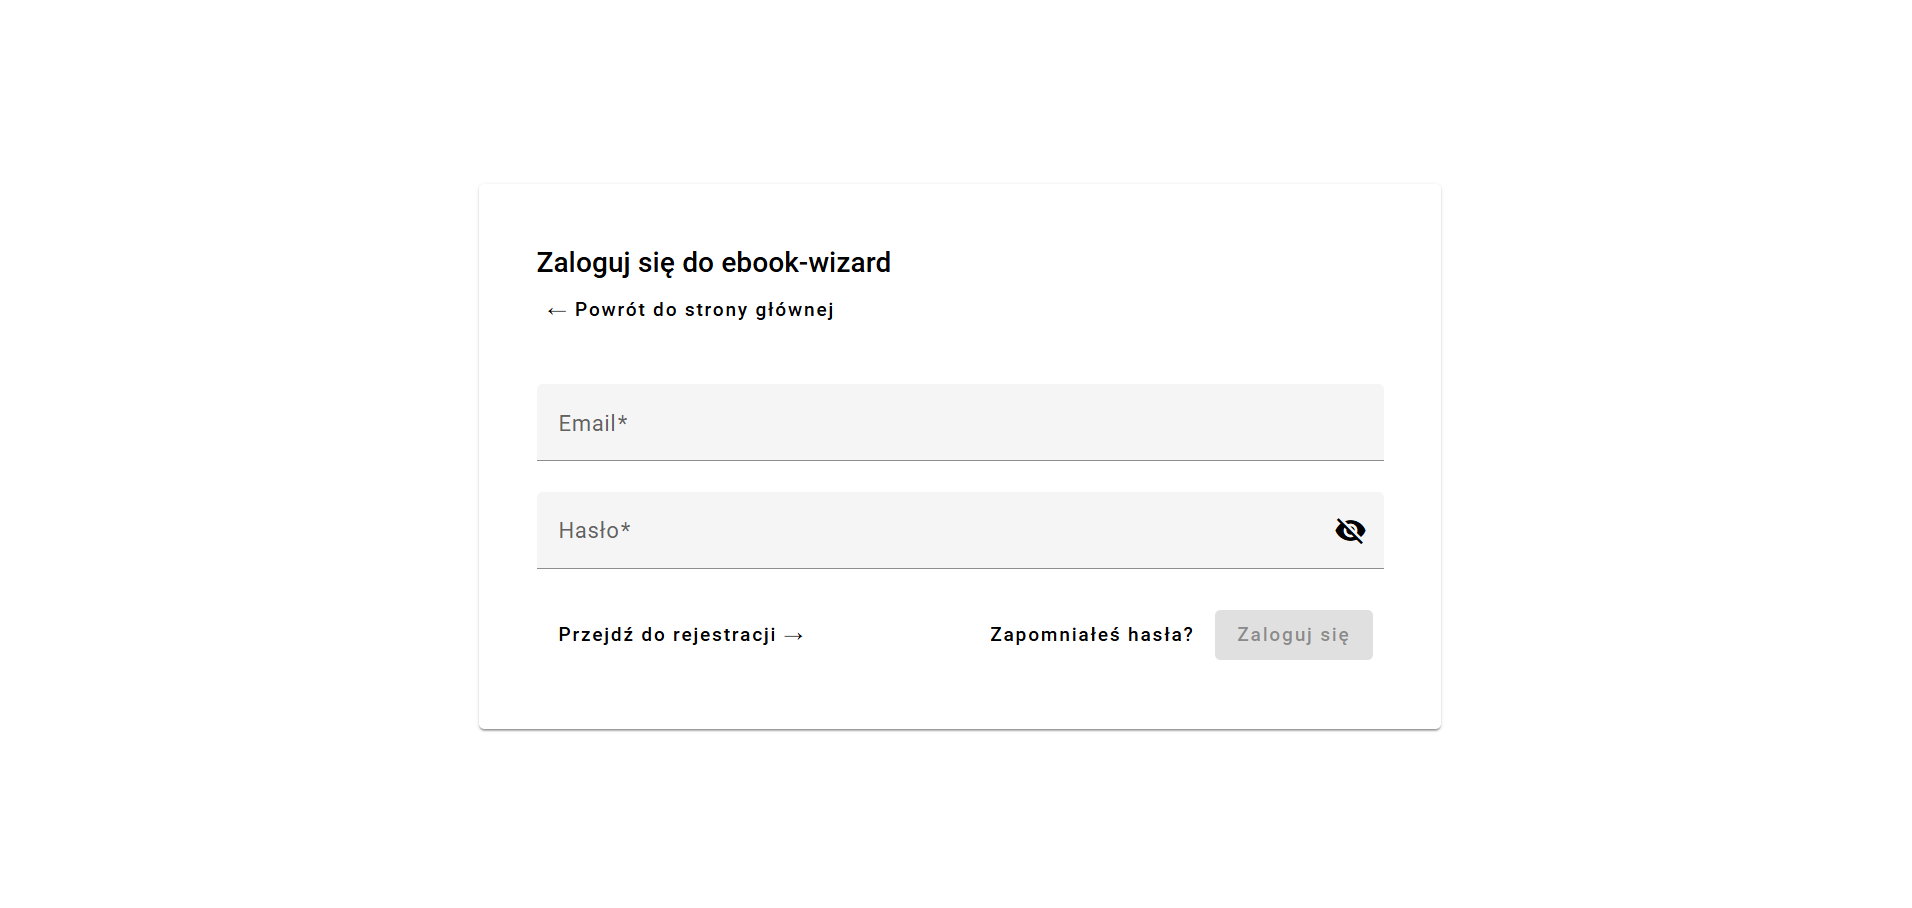
\includegraphics[width=0.9\textwidth]{chap4/page_login.png}}
    \caption{Strona logowania aplikacji Ebook-Wizard}
    \label{fig:page_login}
\end{figure}

\section{Podstrona rejestracji}

Na podstronie rejestracji nowi użytkownicy mogą założyć konto w serwisie.

Zarejestrowanie nowego konta wymaga podania adresu e-mail, pseudonimu oraz hasła. Wymagane jest też zaznaczenie przycisku "Nie jestem robotem" w celu weryfikacji, że konto nie jest zakładane w sposób zautomatyzowany.

Hasło, pseudonim i adres e-mail są walidowane pod względem wymagań. Walidacja jest wykonywana zarówno po stronie frontendu (jeśli formularz jest wypełniony niepoprawnie, przycisk przesłania jest wyłączony), jak i backendu (niepoprawne zapytanie jest odrzucane).

Jeśli użytkownik zacznie wypełniać jakieś pole, wypełni je niepoprawnymi danymi, a następnie przejdzie do następnego pola, pole tekstowe zostanie zaznaczone na czerwono, a pod polem wyświetlona zostanie wiadomość z błędem. Przykład takiego mechanizmu przedstawiono na Rysunku \ref{fig:ebook_wizard_registration_page}. 

Po wypełnieniu formularza, wykonywana jest walidacja adresu e-mailowego. Na podany przez użytkownika adres e-mail zostaje wysłany kod weryfikacyjny, który musi zostać podany w formularzu rejestracji, aby aktywować konto.

\begin{figure}[h]
    \centering
    \setlength{\fboxsep}{0pt}
    \setlength{\fboxrule}{0.4pt}
    \fbox{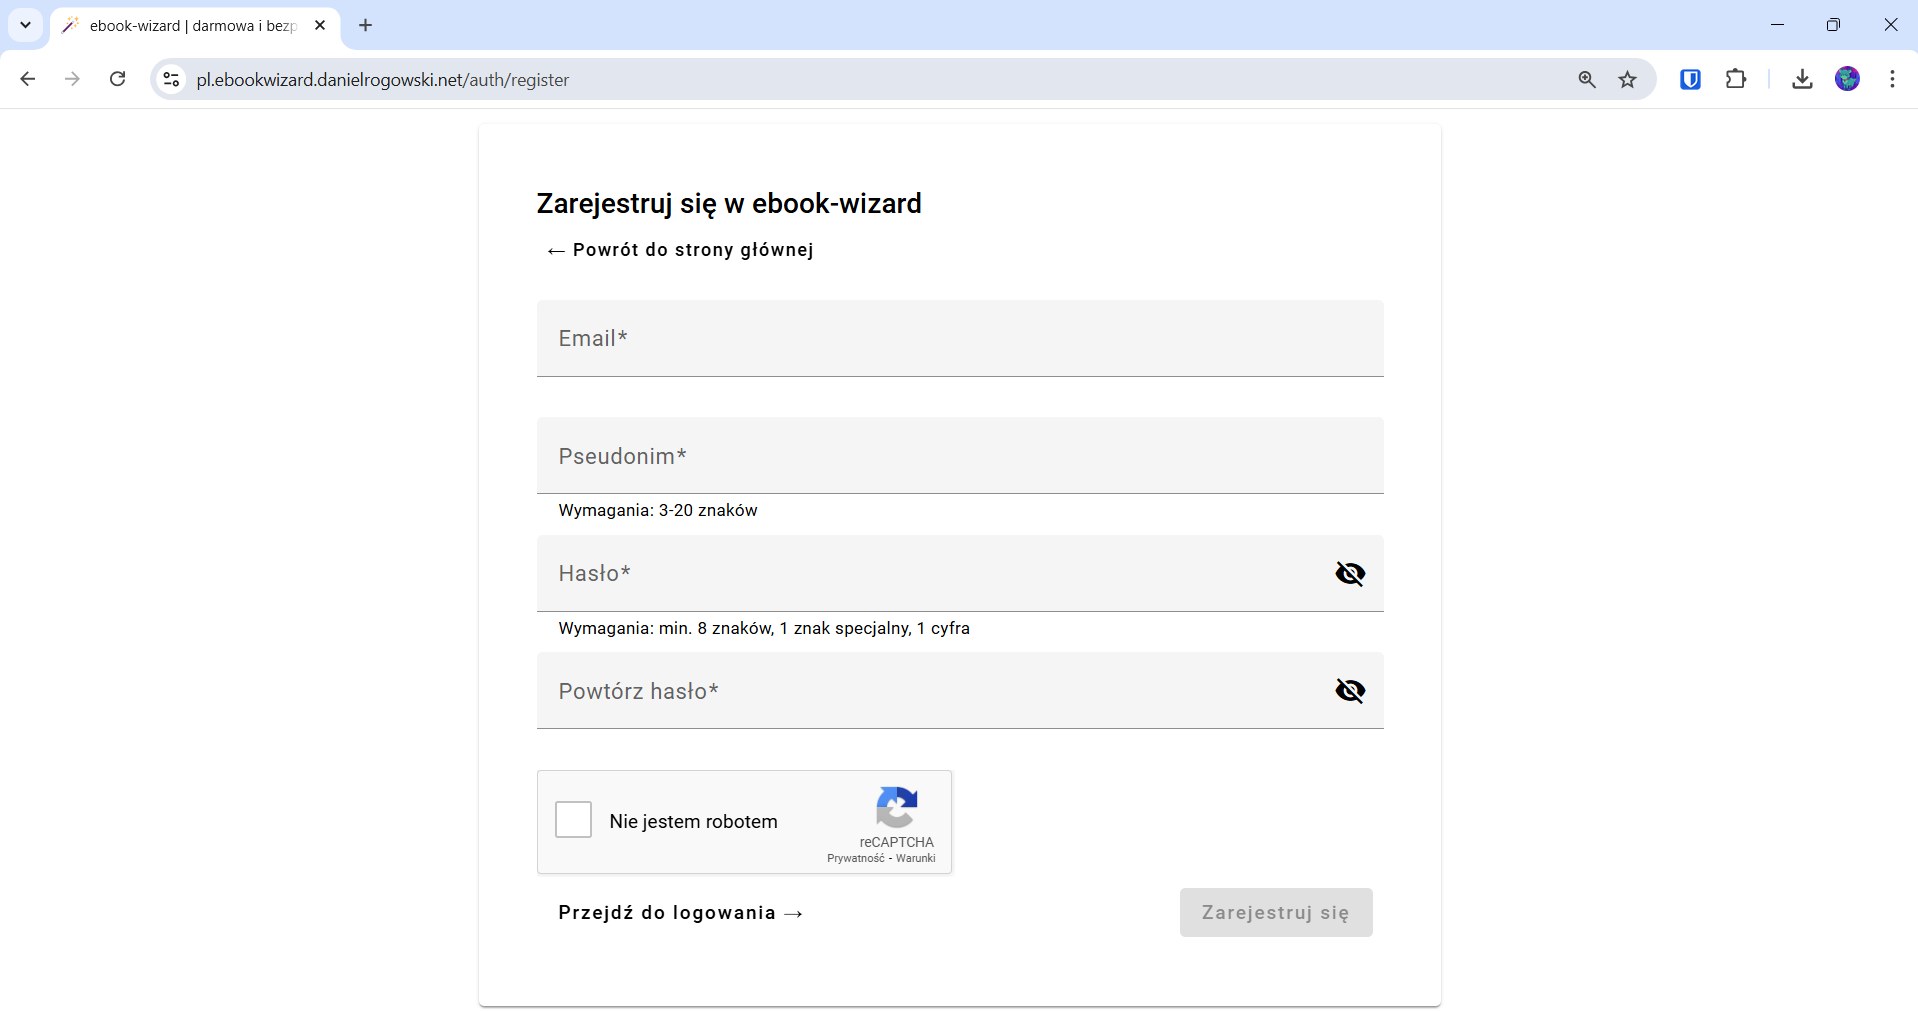
\includegraphics[width=0.9\textwidth]{chap4/page_register.png}}
    \caption{Strona rejestracji aplikacji Ebook-Wizard}
    \label{fig:ebook_wizard_registration_page}
\end{figure}

\section{Podstrona resetowania hasła}

Do podstrony resetowania hasła można przejść klikając przycisk "Zapomniałeś hasło?" widniejący na podstronie logowania. Rozpoczęcie procedury resetu wymaga podania adresu e-mail przypisanego do konta. Zrzut ekranu przedstawiający wygląd podstrony przedstawiono na Rysunku \ref{fig:page_reset_pw}.

Jeśli użytkownik podał poprawny e-mail, otrzyma on na podany adres kod weryfikacyjny, który uprawnia do zmiany hasła na wybrane przez użytkownika.

\begin{figure}[h]
    \centering
    \setlength{\fboxsep}{0pt}
    \setlength{\fboxrule}{0.4pt}
    \fbox{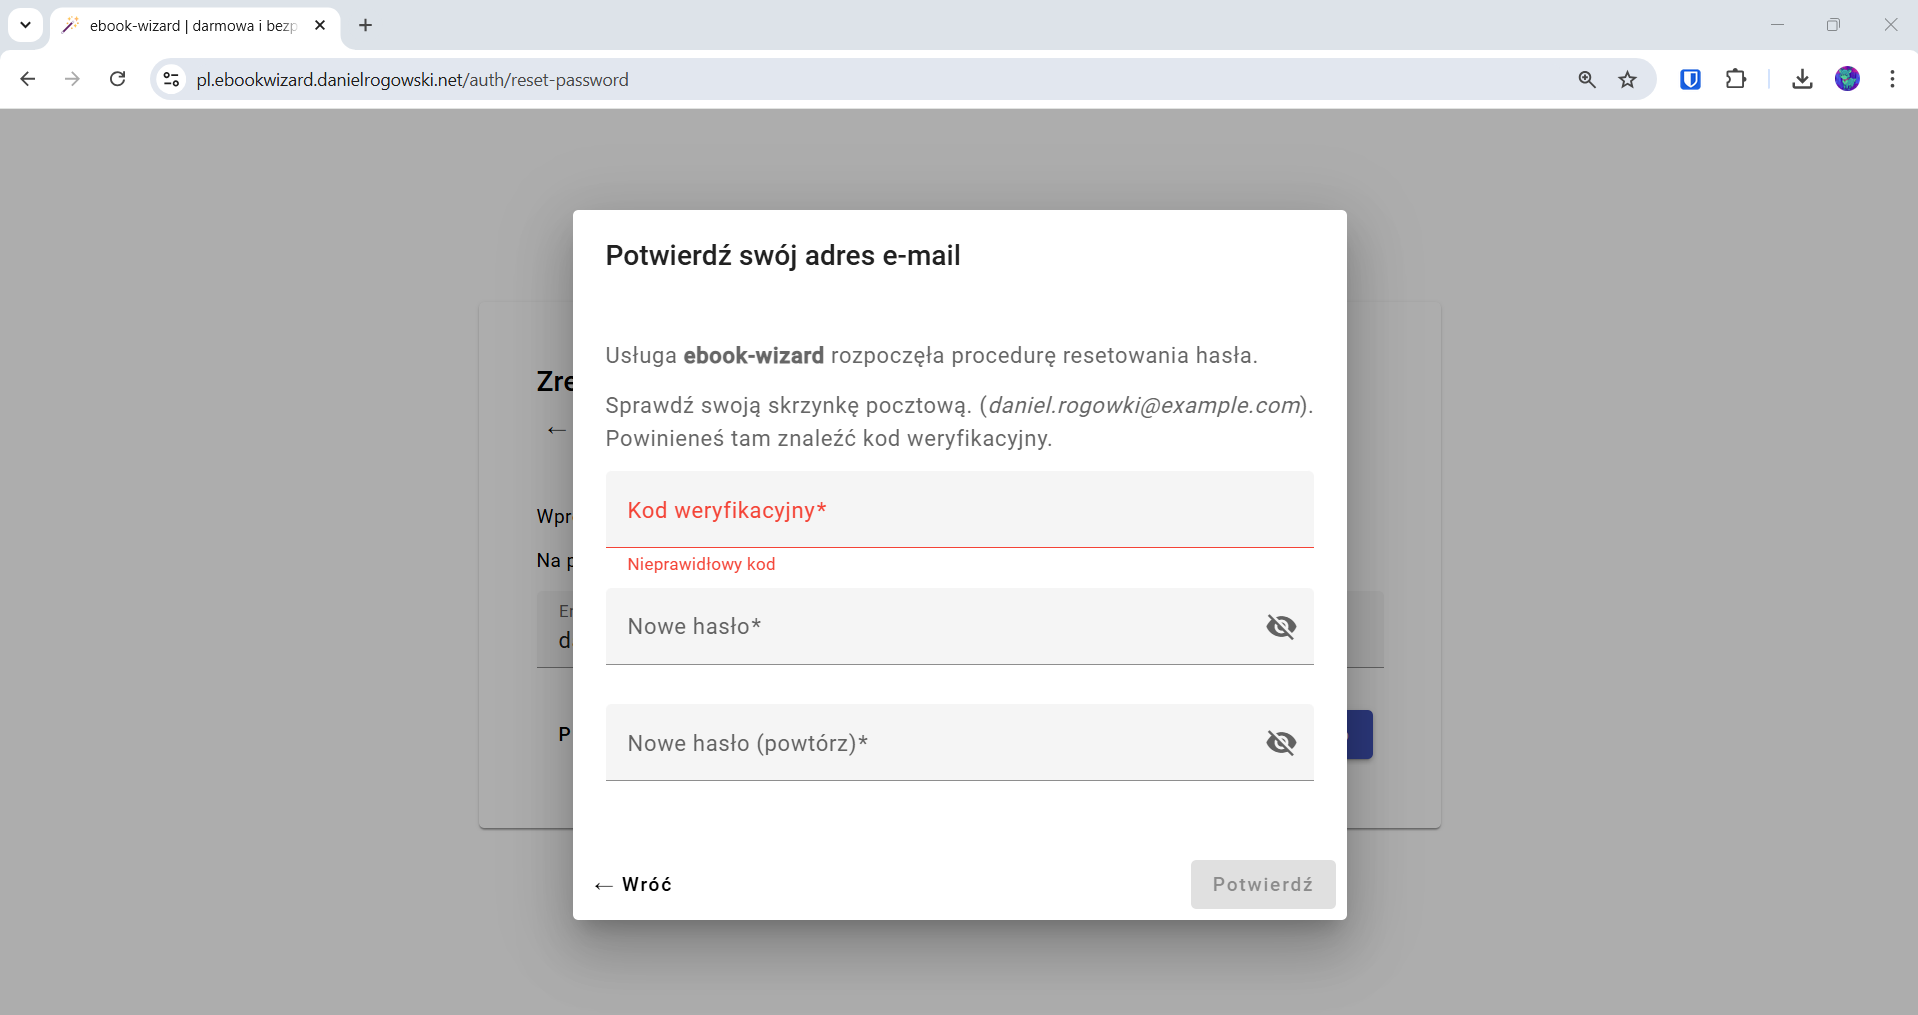
\includegraphics[width=0.9\textwidth]{chap4/page_reset_password.png}}
    \caption{Podstrona resetowania hasła aplikacji Ebook-Wizard}
    \label{fig:page_reset_pw}
\end{figure}

\section{Podstrona zarządzania plikami}

Jest to strona, do której dostęp mają wyłącznie zalogowani użytkownicy. Nawet jeśli użytkownik spróbuje ręcznie wpisać adres URL na pasku przeglądarki, zostanie on przekierowany do strony głównej. Wygląd podstrony zaprezentowano na Rysunku \ref{fig:page_file_management}.

Na podstronie zarządzania plikami użytkownik może zaimportować e-booki, które znajdują się na dysku twardym jego urządzenia, aby następnie wykonywać na nich różnego rodzaju akcje. Opcja importu pozwala na wskazanie pojedynczego pliku lub na zaznaczenie większej ilości plików. Zaimportowanie oznacza przesłanie e-booka na dysk sieciowy usługi Ebook-Wizard.

Podstrona zarządzania plikami nie oferuje możliwości modyfikacji treści e-booka, ani utworzenia e-booka od zera - te opcje są wydzielone do osobnej podstrony, podstrony zarządzania projektami.

Po kliknięciu przycisku "Akcje" na wybranym e-booku, rozwijane jest menu dostępnych akcji. Zawiera ono następujące pozycje:

\begin{itemize}
    \item \textbf{Czytaj} - powoduje przejście do podstrony wyświetlania treści pliku, zawierającej interaktywny czytnik online,
    \item \textbf{Pobierz i konwertuj} - oferuje możliwość przekonwertowania e-booka na jeden ze wspieranych formatów i pobranie wygenerowanego pliku na dysk,
    \item \textbf{Wyślij na czytnik e-booków} - umożliwia przesłanie e-booka na czytnik przy użyciu protokołu e-mailowego,
    \item \textbf{Zmień metadane} - umożliwia skonfigurowanie metadanych, takich jak nazwa i opis e-booka; skonfigurowane metadane zostaną osadzone w pliku, jeśli aktywny format wspiera możliwość osadzania metadanych,
    \item \textbf{Przypisz do folderu} - umożliwia użytkownikowi przeniesienie e-booka do folderu; foldery są wyświetlane w oknie głównym podstrony zarządzania plikami,
    \item \textbf{Zmień obraz okładki} - pozwala na zmianę okładki e-booka poprzez załadowanie pliku graficznego z dysku twardego użytkownika; wskazana okładka wyświetlana jest zarówno w menu aplikacji Ebook-Wizard, jak i zostaje osadzona w metadanych pliku (jeśli aktywny format wspiera możliwość osadzania metadanych),
    \item \textbf{Usuń} - usuwa plik wraz ze wszystkimi jego formatami, zwalniając przestrzeń dyskową którą zajmował,
    \item \textbf{Konwertuj do projektu} - umożliwia przekonwertowanie pliku na projekt, tym samym umożliwiając modyfikację treści danego e-booka,
    \item \textbf{Udostępnij} - pozwala na wygenerowanie hiperłącza do e-booka, które następnie można przekazać innym osobom w celu podzielenia się e-bookiem.
\end{itemize}

\begin{figure}[h]
    \centering
    \setlength{\fboxsep}{0pt}
    \setlength{\fboxrule}{0.4pt}
    \fbox{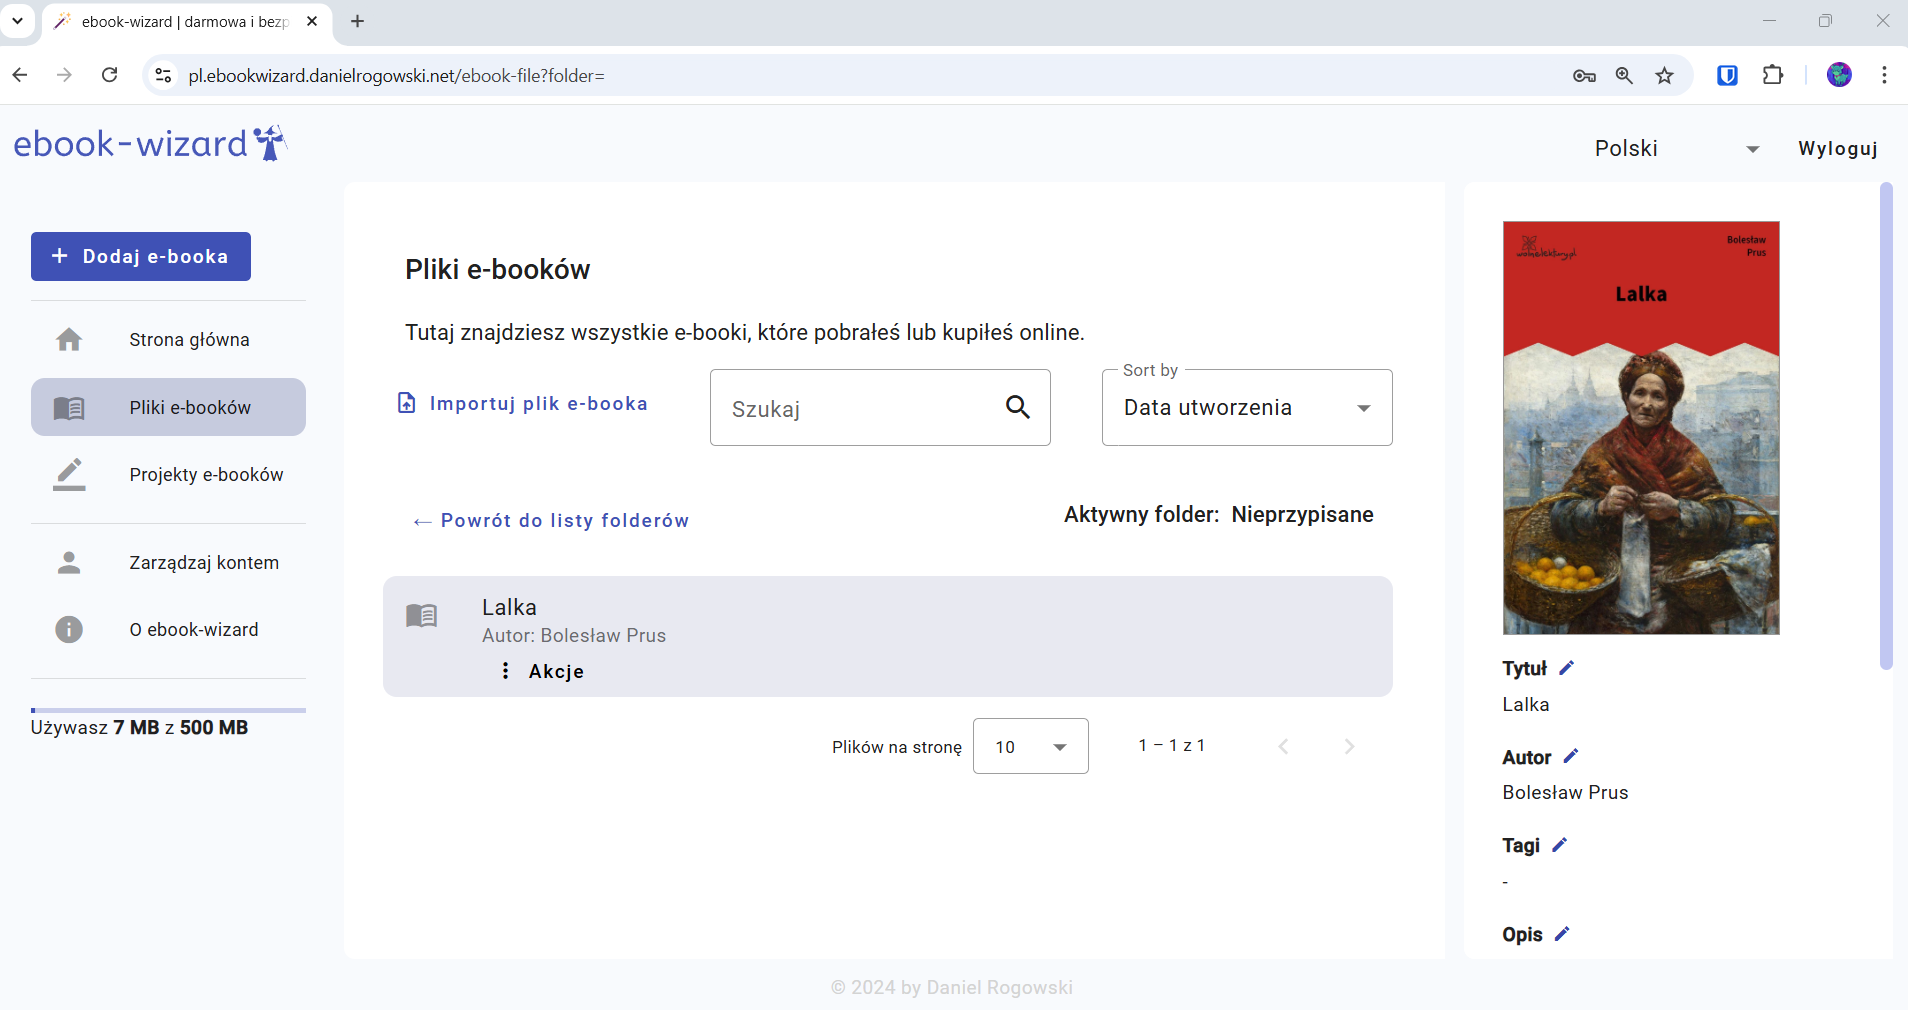
\includegraphics[width=0.9\textwidth]{chap4/page_ebook_page.png}}
    \caption{Podstrona zarządzania plikami aplikacji Ebook-Wizard}
    \label{fig:page_file_management}
\end{figure}

\section{Podstrona zarządzania projektami}

Podstrona zarządzania projektami pozwala na stworzenie nowego e-booka oraz wypełnienie go zawartością tekstową i graficzną. Różni się więc od podstrony zarządzania plikami, która służyła do zarządzania już istniejącymi e-bookami. Graficzny interfejs podstrony został pokazany na Rysunku \ref{fig:page_project_management}.

Na tej podstronie nie ma opcji importu z pliku. Znajduje się natomiast przycisk "Utwórz projekt e-booka", który pozwala stworzyć nowego e-booka od podstaw. Formularz tworzenia e-booka pozwala skonfigurować metadane oraz obraz okładki.

Po kliknięciu przycisku "Akcje" na wybranym e-booku, rozwijane jest menu dostępnych akcji. Zawiera ono następujące pozycje:

\begin{itemize}
    \item \textbf{Edytuj} - powoduje przejście do podstrony edytora projektu, zawierającej interaktywny edytor WYSIWYG,
    \item \textbf{Modyfikuj metadane} - zmiana metadanych takich jak nazwa, opis czy tagi,
    \item \textbf{Zmień obraz okładki} - pozwala na dodanie pliku graficznego, który będzie stanowił obraz okładki,
    \item \textbf{Pobierz} - zapisuje projekt do postaci jednego ze wspieranych formatów i pozwala na pobranie pliku na dysk twardy użytkownika,
    \item \textbf{Konwertuj do pliku} - przenosi projekt z podstrony zarządzania projektami do podstrony zarządzania plikami,
    \item \textbf{Usuń} - usuwa projekt, wszystkie przypisane do niego ilustracje, i zwalnia przestrzeń dyskową która była zajmowana przez projekt, 
    \item \textbf{Wyślij na czytnik e-booków} - zapisuje projekt do postaci jednego ze wspieranych formatów i pozwala na przesłanie go na czytnik przy użyciu protokołu e-mailowego,
    \item \textbf{Udostępnij} - umożliwia wygenerowanie hiperłącza, które pozwala innym użytkownikom na przeczytanie e-booka.
\end{itemize}

\begin{figure}[h]
    \centering
    \setlength{\fboxsep}{0pt}
    \setlength{\fboxrule}{0.4pt}
    \fbox{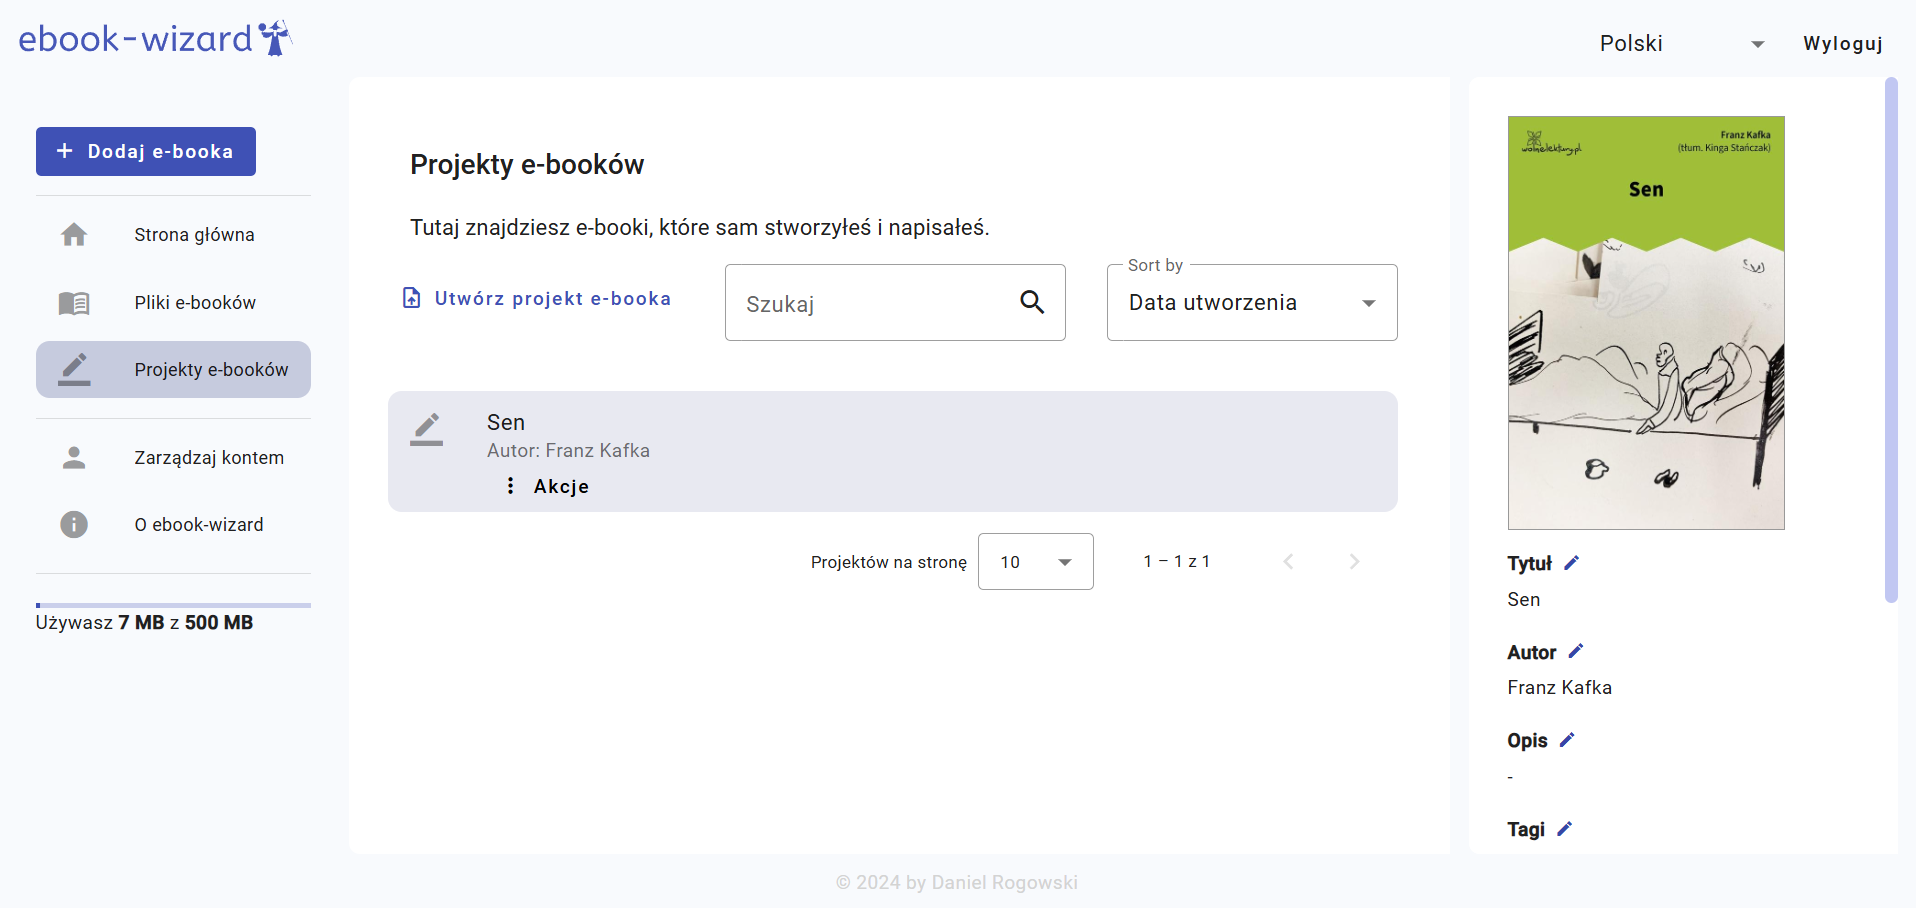
\includegraphics[width=0.9\textwidth]{chap4/page_ebook_project_page.png}}
    \caption{Podstrona zarządzania projektami aplikacji Ebook-Wizard}
    \label{fig:page_project_management}
\end{figure}

\section{Podstrona edytora projektu}

Do tej podstrony można przejść poprzez wybranie akcji "Edytuj" na wybranym projekcie e-booka. Edytor projektu oferuje możliwość modyfikacji zawartości e-booka. Wygląd edytora zaprezentowano na Rysunku \ref{fig:page_project_editor}.

Po lewej stronie edytora znajduje się edytor rozdziałów. Pozwala on na tworzenie rozdziału, modyfikowanie nazw, usuwanie, a także zmienianie kolejności rozdziałów przy użyciu metody "przeciągnij i upuść". Gdy projekt jest eksportowany na dysk twardy użytkownika, rozdziały zdefiniowane w edytorze są osadzane w metadanych pliku jako spis treści (o ile wybrany format wspiera taką możliwość). Niektóre fizyczne czytniki e-booków (np. Amazon Kindle) potrafią odczytać ten spis treści i wyświetlać go w menu czytnika.

Prawa strona edytora zawiera natomiast edytor WYSIWYG, pozwalający na dodanie zawartości do wybranego rozdziału. Możliwe jest dodawanie tekstu oraz ilustracji z dysku twardego. Edytor wspiera możliwość zmiany formatowania tekstu (np. pogrubienie, pochylenie, podkreślenie, zmiana kroju czcionki).

\begin{figure}[h]
    \centering
    \setlength{\fboxsep}{0pt}
    \setlength{\fboxrule}{0.4pt}
    \fbox{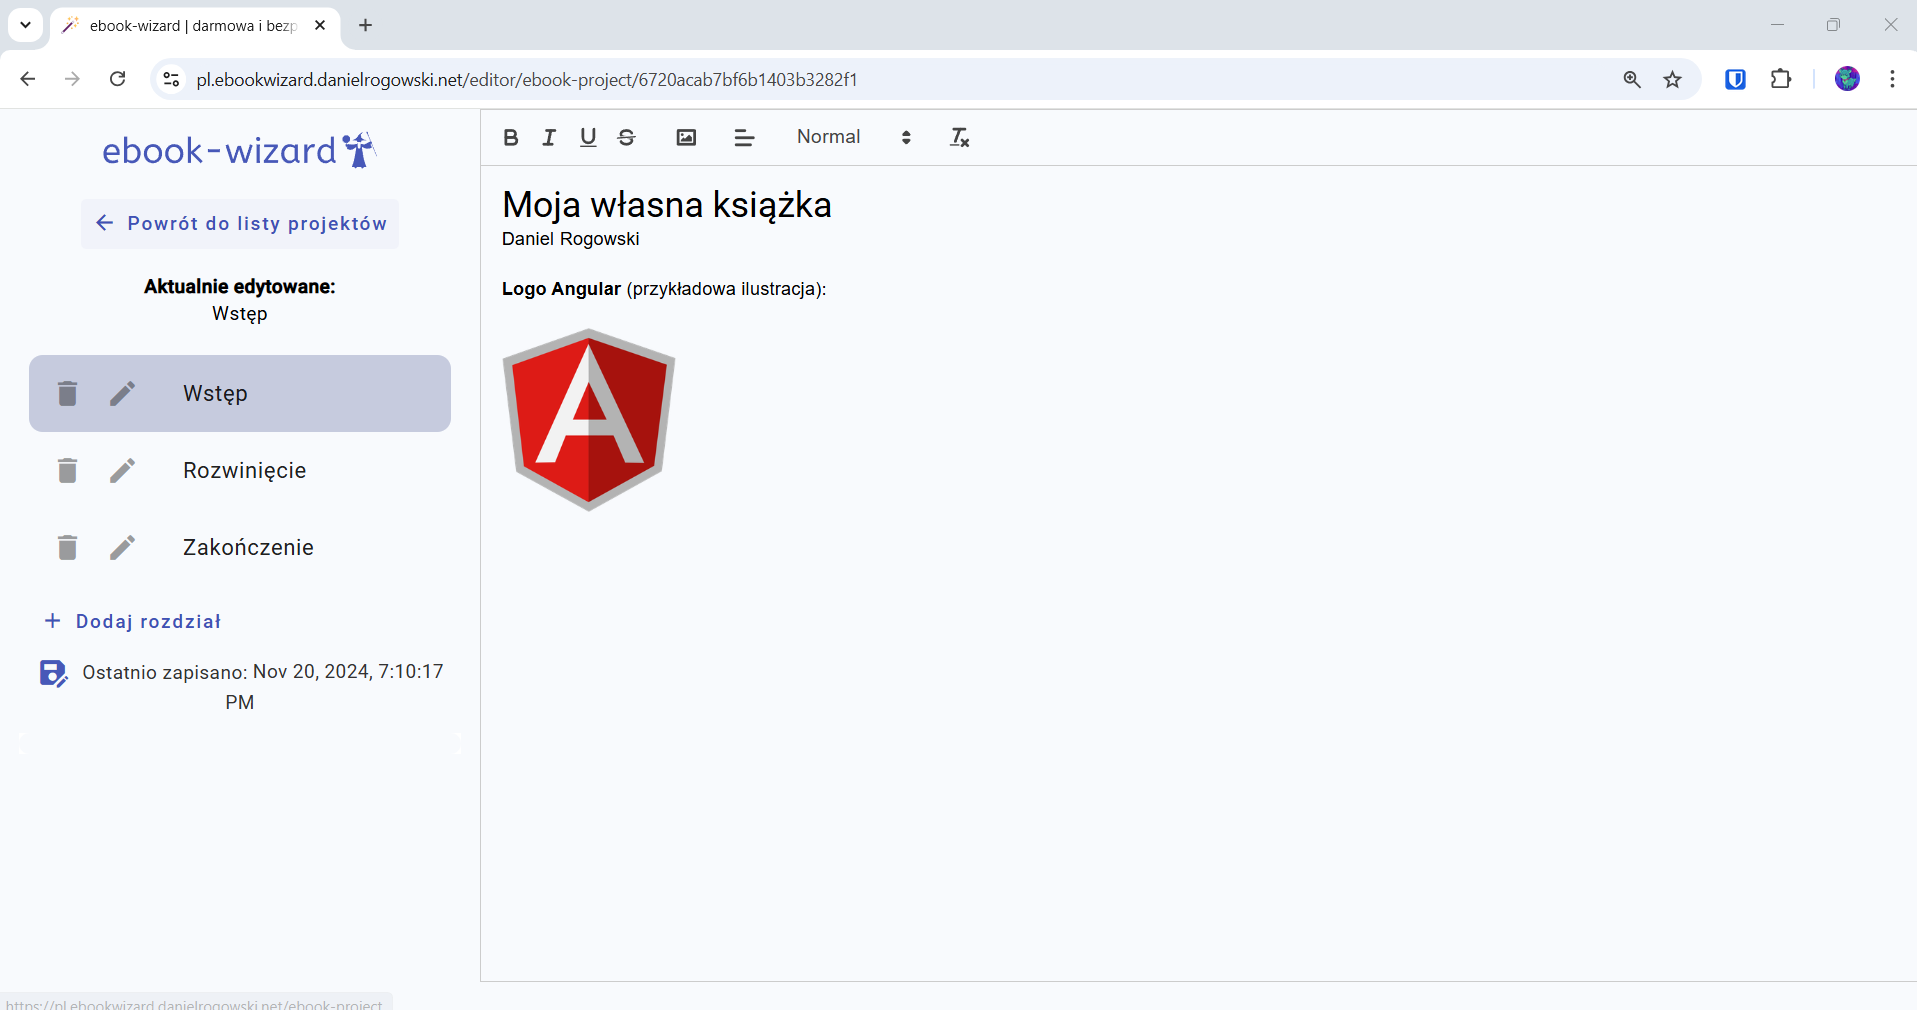
\includegraphics[width=0.9\textwidth]{chap4/page_project_editor.png}}
    \caption{Podstrona edytowania projektu aplikacji Ebook-Wizard}
    \label{fig:page_project_editor}
\end{figure}

\section{Podstrona wyświetlania treści pliku}

Do tej podstrony można przejść wybierając akcję "Czytaj" na wybranym e-booku na podstronie zarządzania plikami. Na tej podstronie znajduje się interaktywny czytnik, pozwalający na przeglądanie zawartości e-booka bezpośrednio w przeglądarce. Wygląd wspomnianego czytnika zaprezentowano na Rysunku \ref{fig:page_file_display}.

Na prawo od wyświetlanej strony, aplikacja Ebook-Wizard wyświetla kilka przycisków kontrolnych:
\begin{itemize}
    \item \textbf{Zmiana strony} - przyciski przenoszące do poprzedniej i aktualnej strony; jeśli operacja jest niemożliwa (na przykład dotarto na koniec e-booka), odpowiedni przycisk zostaje wyłączony
    \item \textbf{Zakładki} - możliwość zapisania aktualnie wyświetlanej strony w zakładkach; możliwość powrotu do wcześniej zapisanych stron
    \item \textbf{Generowanie audiobooka} - automatyczne czytanie zawartości ekranu przez model sztucznej inteligencji dostarczany przez usługę Amazon Polly
\end{itemize}

\begin{figure}[h]
    \centering
    \setlength{\fboxsep}{0pt}
    \setlength{\fboxrule}{0.4pt}
    \fbox{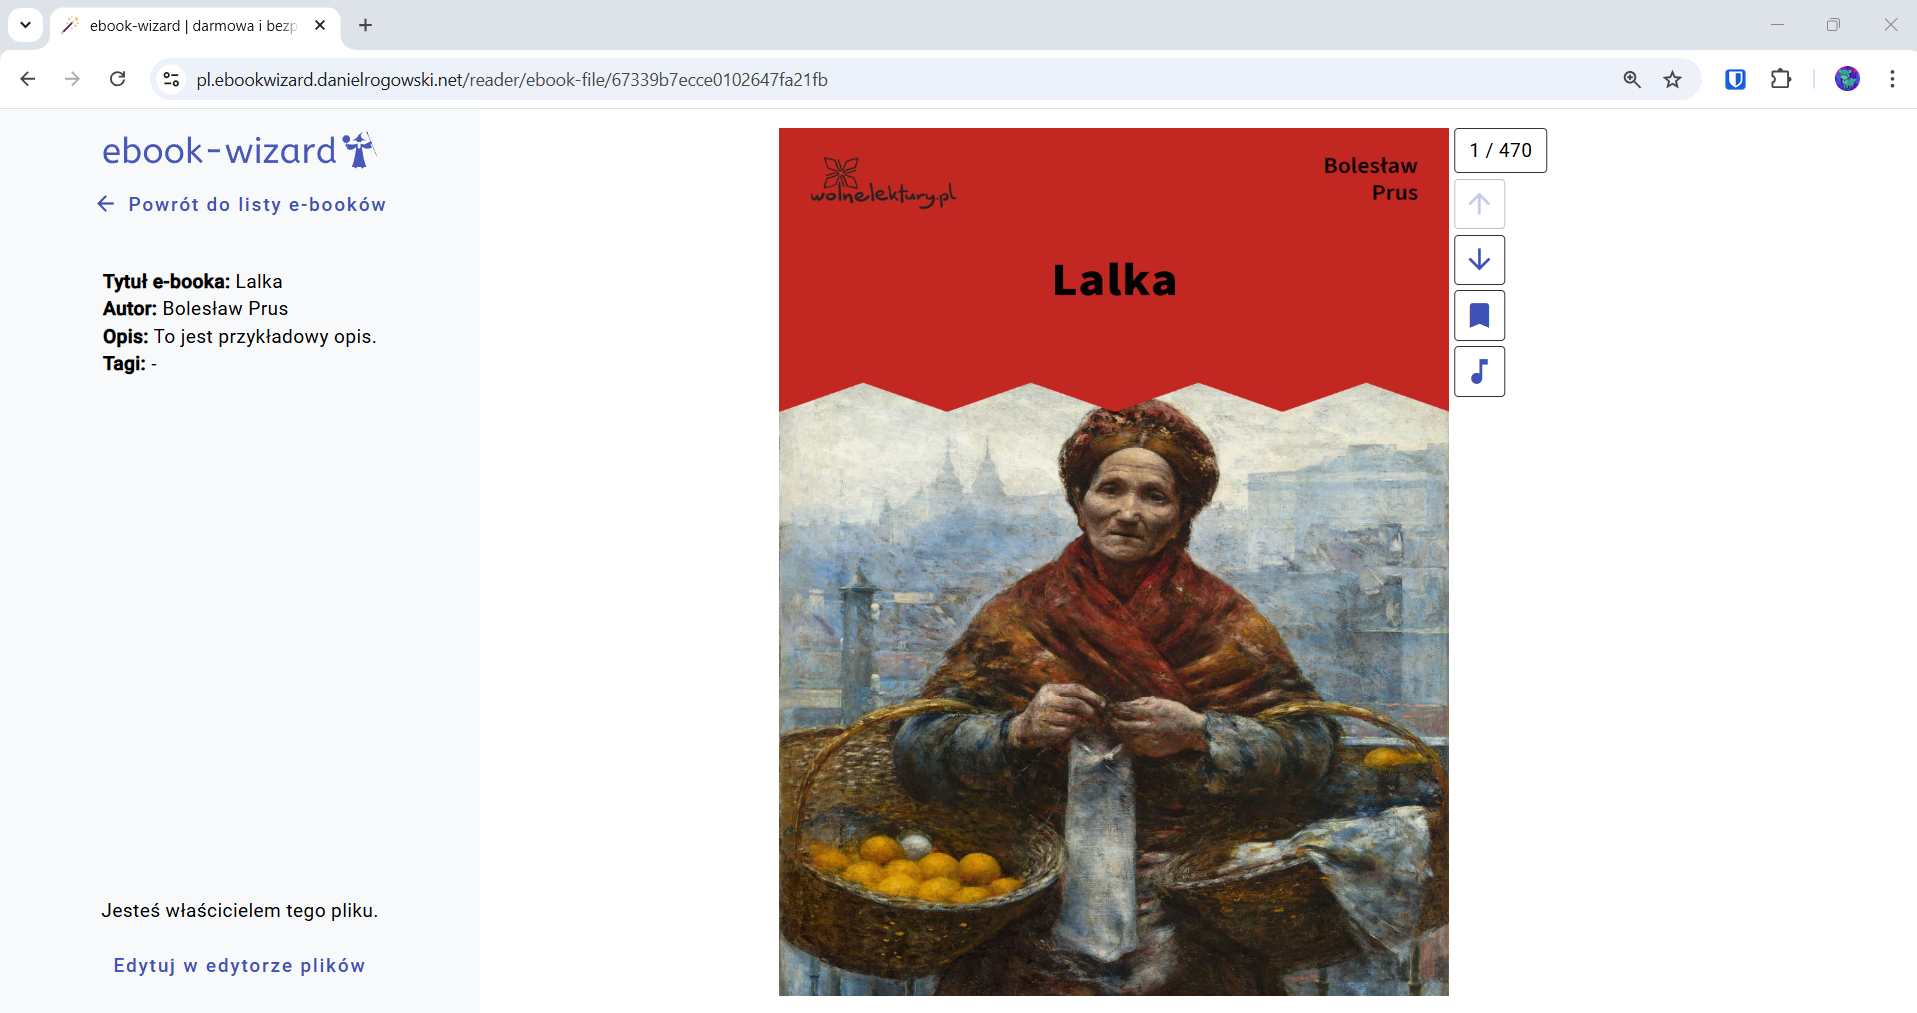
\includegraphics[width=0.9\textwidth]{chap4/page_ebook_display.png}}
    \caption{Podstrona wyświetlania treści pliku aplikacji Ebook-Wizard}
    \label{fig:page_file_display}
\end{figure}

\section{Podstrona zarządzania kontem}

Na tej podstronie wyświetlane są podstawowe informacje na temat konta użytkownika. Oferowana jest też możliwość zmiany adresu e-mail, pseudonimu oraz hasła, a także opcja trwałego usunięcia konta.

Do podstrony zarządzania kontem można przejść z poziomu podstrony zarządzania plikami lub projektami, klikając przycisk "Zarządzaj kontem" znajdujący się po lewej stronie ekranu.

Wygląd podstrony zarządzania kontem przedstawiono na Rysunku \ref{fig:page_account_mngmt}.

\begin{figure}[h]
    \centering
    \setlength{\fboxsep}{0pt}
    \setlength{\fboxrule}{0.4pt}
    \fbox{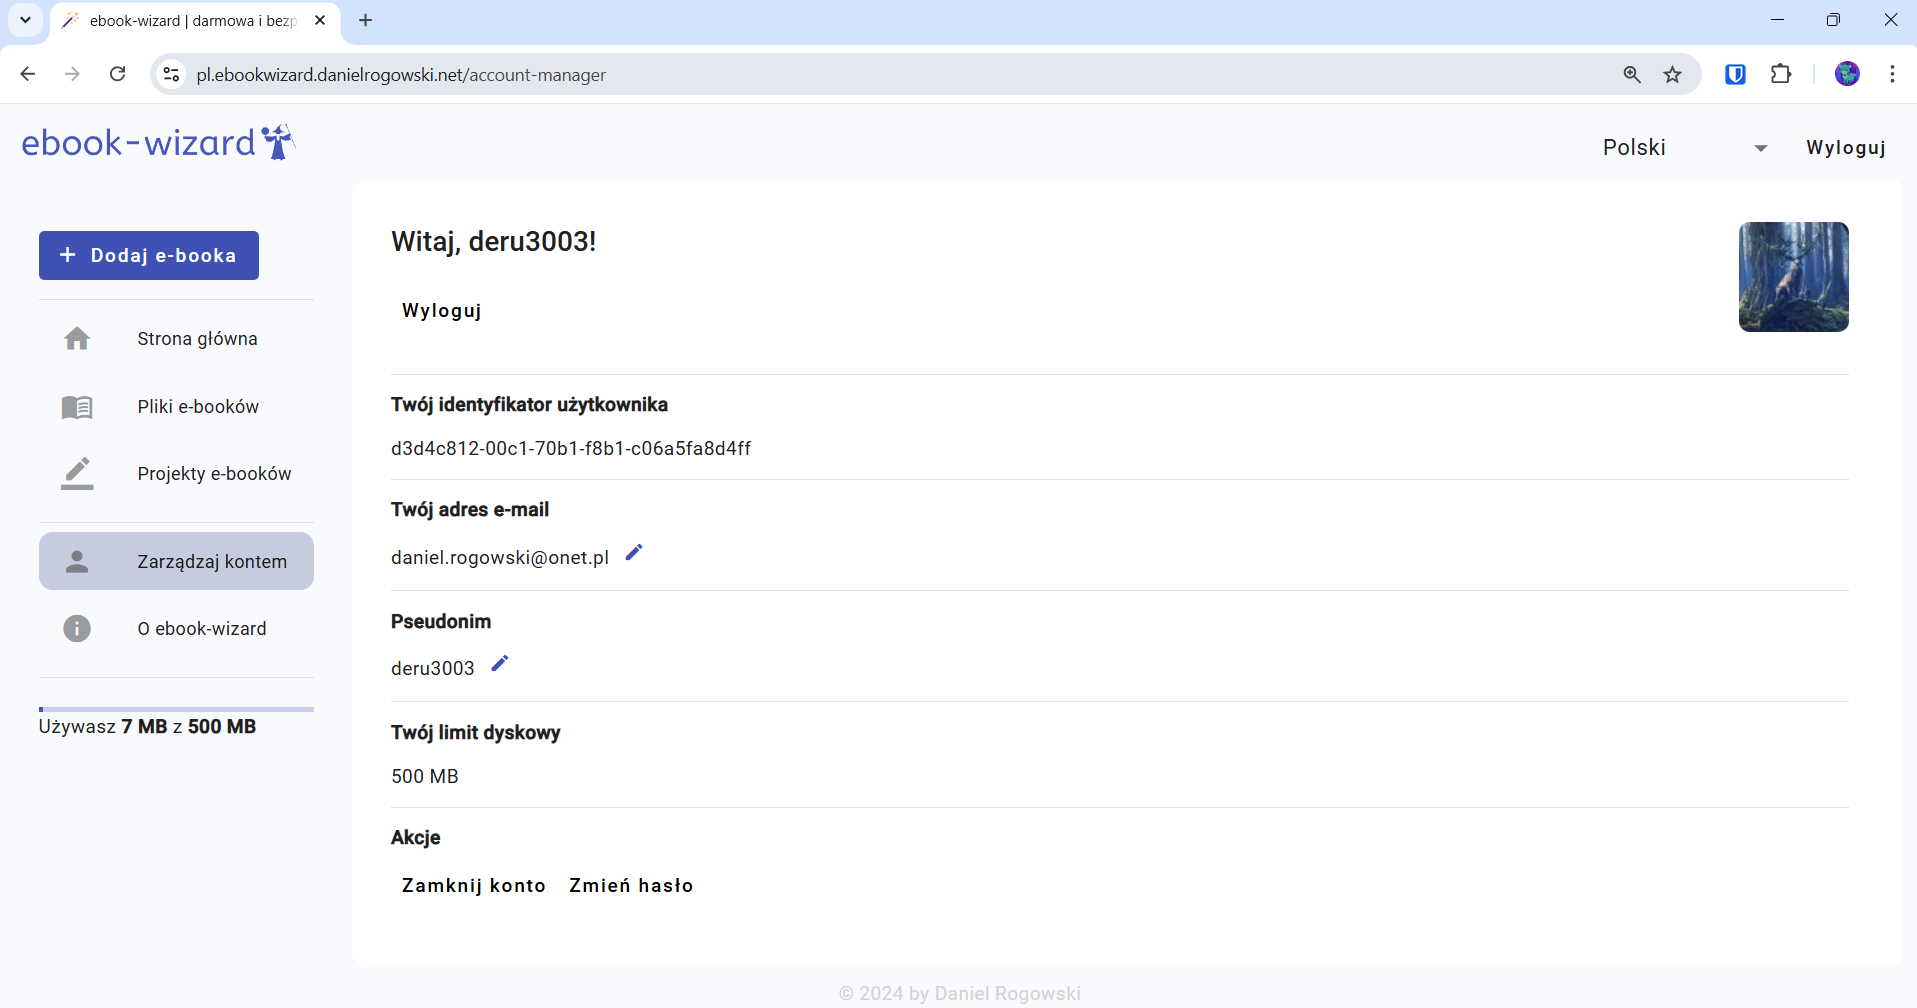
\includegraphics[width=0.9\textwidth]{chap4/page_account_mngmnt.png}}
    \caption{Podstrona zarządzania kontem aplikacji Ebook-Wizard}
    \label{fig:page_account_mngmt}
\end{figure}

\section{Podstrona regulaminu i statystyk}

Do podstrony regulaminu i statystyk można przejść klikając przycisk "O Ebook-Wizard" z poziomu podstrony zarządzania plikami lub projektami. Hiperłącze do regulaminu znajduje się również w stopce strony głównej. Wygląd podstrony przedstawiono na Rysunku \ref{fig:page_stats}.

Na podstronie znajdują się dwie zakładki. Pierwsza z nich, zatytułowana "Regulamin", wyświetla listę zasad serwisu Ebook-Wizard. Niestosowanie się do tych reguł może skutkować zawieszeniem konta. 

Druga zakładka, "Panel statystyk", wyświetla globalne statystyki aplikacji Ebook-Wizard. Na tej podstronie wyświetlana jest globalna liczba użytkowników, plików oraz projektów.

Ponadto, na podstronie regulaminu i statystyk wyświetlane jest poziome menu nawigacyjne, umożliwiające przejście do strony głównej oraz do edytora e-booków.

\begin{figure}[h]
    \centering
    \setlength{\fboxsep}{0pt}
    \setlength{\fboxrule}{0.4pt}
    \fbox{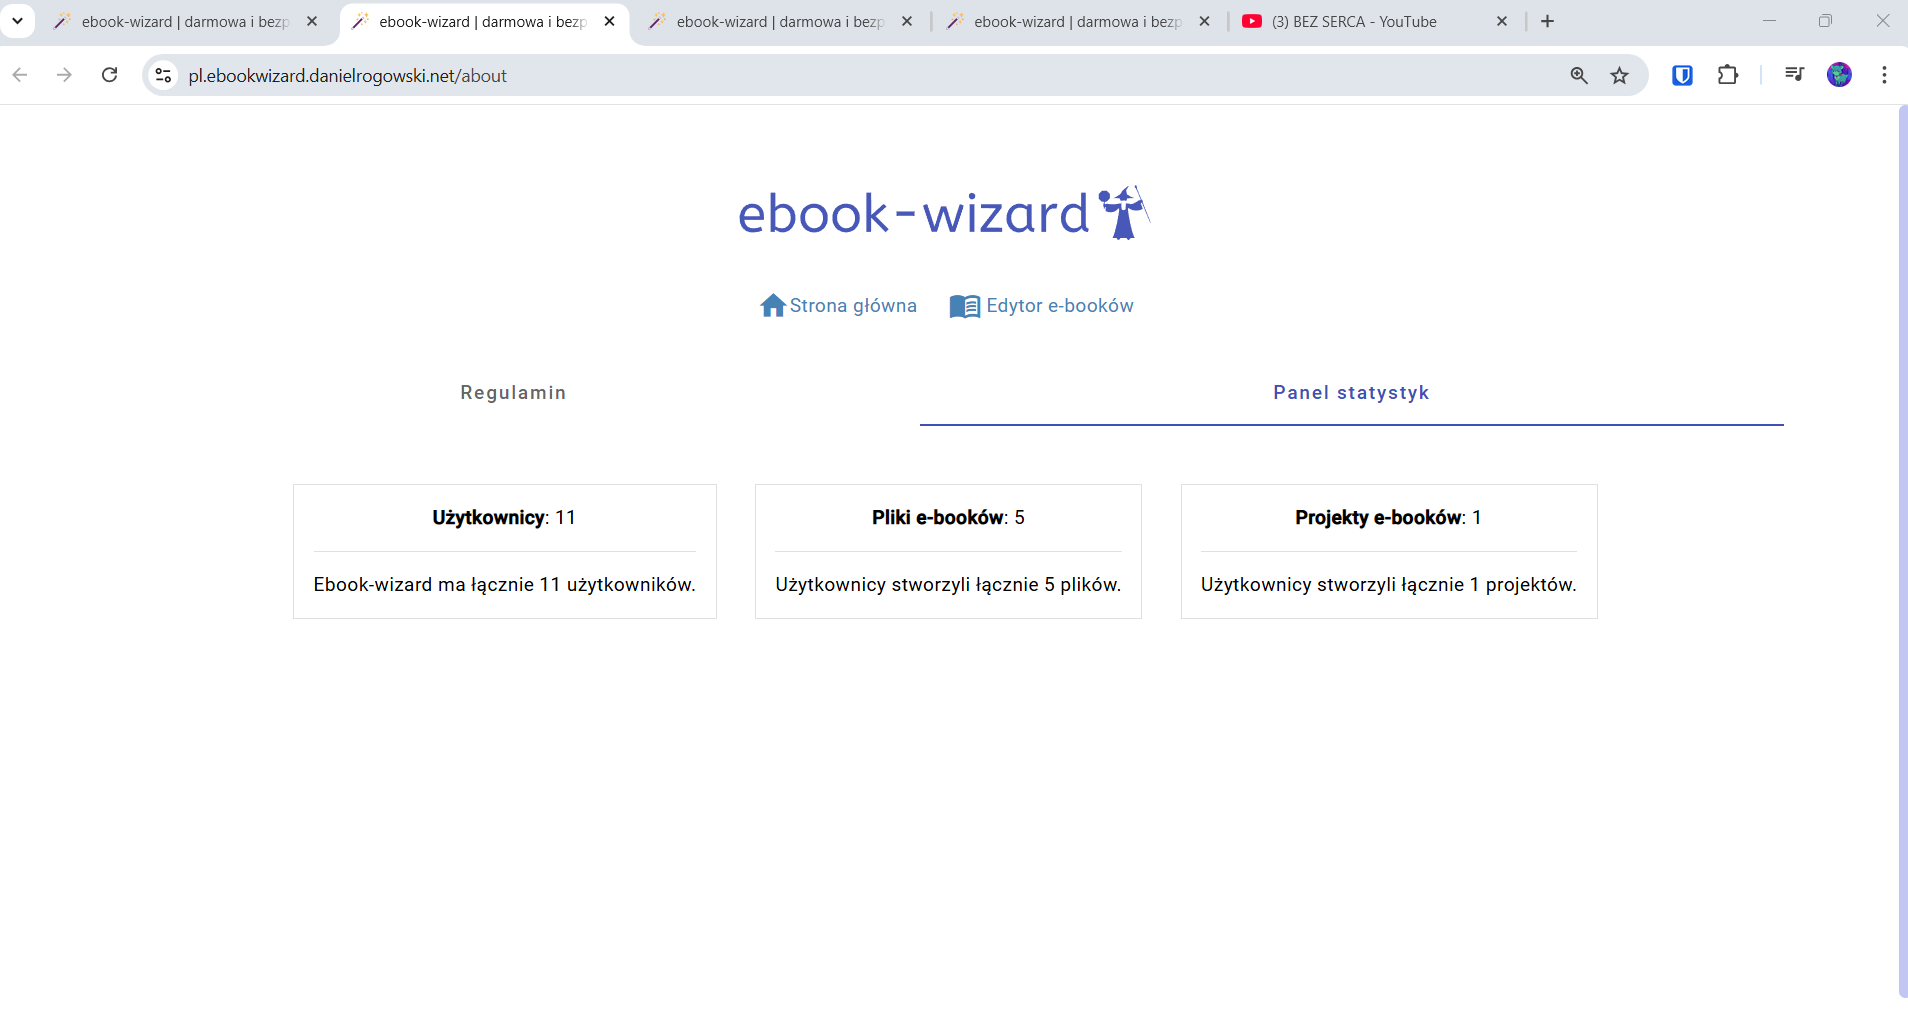
\includegraphics[width=0.9\textwidth]{chap4/page_stats.png}}
    \caption{Podstrona regulaminu i statystyk aplikacji Ebook-Wizard}
    \label{fig:page_stats}
\end{figure}

\section{Podstrona informacji o błędzie}

W przypadku, gdy użytkownik spróbuje wyświetlić podstronę o nieistniejącej ścieżce URL, zostanie on przekierowany do podstrony wyświetlającej informację o błędzie HTTP 404.

Na podstronie z informacją o błędzie znajduje się wyjaśnienie przyczyny błędu oraz przycisk pozwalający na powrót do strony głównej.

% \begin{figure}[h]
%     \centering
%     \setlength{\fboxsep}{0pt}
%     \setlength{\fboxrule}{0.4pt}
%     \fbox{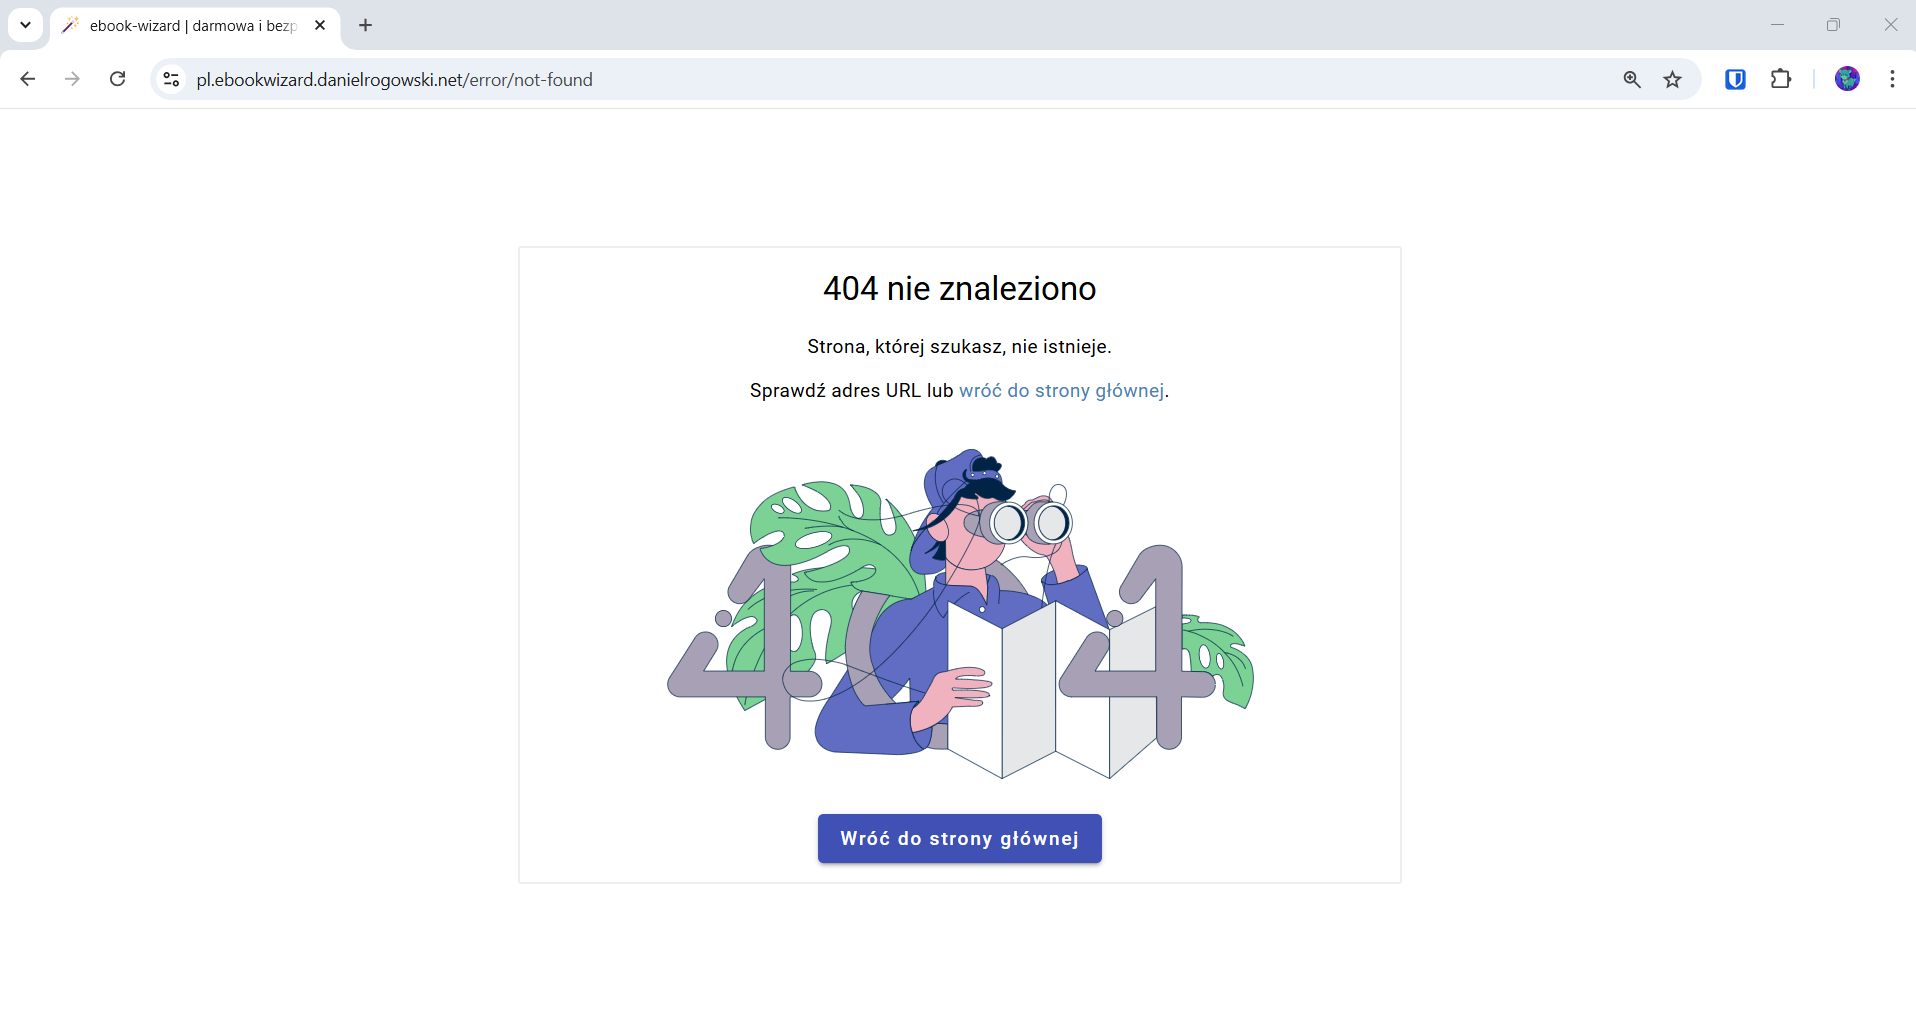
\includegraphics[width=0.9\textwidth]{chap4/page_404.png}}
%     \caption{Podstrona informacji o błędzie aplikacji Ebook-Wizard}
%     \label{fig:obrazek_z_ramką}
% \end{figure}
